\begin{enumerate}[label=\arabic*.,ref=\theenumi]
%\begin{enumerate}[label=\thesection.\arabic*.,ref=\thesection.\theenumi]
\numberwithin{equation}{enumi}

\item

For the circuit in Fig. \ref{fig:ee18btech11051_fig1}, break the loop at node X and find the loop gain (working backward for simplicity to find $V_{X}$ in terms of $V_{O}$). For R = 10 k$\ohm$, find C and $R_{f}$ to obtain sinusoidal oscillations at 10 kHz.

\begin{figure}[!ht]
	\begin{center}
		\resizebox{\columnwidth}{!}{\begin{circuitikz}
\ctikzset{bipoles/length=1cm}

 
\draw (0, 0) node[op amp, scale = 0.5] (opamp) {};
\draw (opamp.-) --(-1,0.25)-- (-1,1) to[R=$R_{f}$,*-*] (1,1) -- (1,0);%[C=$C$,*-*] (0.25,-1) to [R=$R$,*-*] (-1,-1) -- (-1,-0.35) to (opamp.+);
\draw (opamp.+) --(-1,-0.25) to node[ground]{}  (-1, -0.6) ;
\draw (-1, 0.25) to [R=$R$,*-*] (-2.6, 0.25) to [C=$C$,*-*] (-2.6, -1.5) to node[ground]{} (-2.6,-2);
\draw (-2.6, 0.25) to [R=$R$,*-*] (-3.9, 0.25) to [C=$C$,*-*] (-3.9, -1.5) to node[ground]{} (-3.9,-2);
\draw (-3.9, 0.25) to [R=$R$,*-*] (-5.2, 0.25) to [C=$C$,*-*] (-5.2, -1.5) to node[ground]{} (-5.2,-2);
\draw (-5.2, 0.25) to [R=$R$,*-*] (-6.5, 0.25) -- (-6.5, 2) -- (1,2)-- (1,1);
\draw (opamp.out) -- (1.5,0) ;
\draw node at (1.8, 0){$V_{O}$};
\draw node at (-6.8, 0.25){X};
\end{circuitikz}
}
	\end{center}
\caption{}
\label{fig:ee18btech11051_fig1}
\end{figure}

\item
\solution
We first calculate the relation between $I_{4}$ and $V_{X}$ in fig \ref{fig:ee18btech11051_fig2} by using the relation between the currents and the fact that the inverting terminal of the Op-Amp is virtually grounded as follows:
\begin{figure}[!ht]
	\begin{center}
		\resizebox{\columnwidth}{!}{\begin{circuitikz}
\ctikzset{bipoles/length=1cm}


\draw (0, 0.25) to [C=$C$,*-*] (0, -1.5) to node[ground]{} (0,-2);
\draw (0, 0.25) to [R=$R$,*-*] (-2, 0.25) to [C=$C$,*-*] (-2, -1.5) to node[ground]{} (-2,-2);
\draw (-2, 0.25) to [R=$R$,*-*] (-4, 0.25) to [C=$C$,*-*] (-4, -1.5) to node[ground]{} (-4,-2);
\draw (-4, 0.25) to [R=$R$,*-*] (-6, 0.25);
\draw (0, 0.25) to [R=$R$,*-*] (2, 0.25);

\draw[-latex] (-6,0.25) to node[below] {$I_{1}$} (-5.6, 0.25);
\draw[-latex] (-4,0.25) to node[below] {$I_{2}$} (-3.6, 0.25);
\draw[-latex] (-2,0.25) to node[below] {$I_{3}$} (-1.6, 0.25);
\draw[-latex] (0,0.25) to node[below] {$I_{4}$} (0.4, 0.25);

\draw node at (-4, 0.5){$V_{1}$};
\draw node at (-2, 0.5){$V_{2}$};
\draw node at (0, 0.5){$V_{3}$};
\draw node at (2, 0.5){$V_{4}$};
\draw node at (-6, 0.5){$V_{X}$};
\end{circuitikz}
}
	\end{center}
\caption{}
\label{fig:ee18btech11051_fig2}
\end{figure}

Here, $V_{4}$ has zero voltage. Applying KVL between $V_{3}$ and $V_{4}$, we get
\begin{align}
    V_{3} = I_{4}R \label{eq:ee18btech11051_0}
\end{align}

Starting at node $V_{3}$ to node $V_{X}$, applying KCL and KVL sequentially, and substituting the previous two equations gives:\\
\begin{multline}
    I_{3} = I_{4} + V_{3}sC  \\  \implies I_{3} = I_{4}(1+sRC) 
\end{multline}
\begin{multline}
    V_{2} = V_{3} + I_{3}R  \\  \implies V_{2} = I_{4}R(2+sRC)
\end{multline}
\begin{multline}
    I_{2} = I_{3} + V_{2}sC\\
    \implies I_{2} = I_{4}(1+3sRC+(sRC)^{2}) 
\end{multline}
\begin{multline}
    V_{1} = V_{2}+ I_{2}R\\
    \implies V_{1} = I_{4}R(3+4sRC+(sRC)^{2})
\end{multline}
\begin{multline}
    I_{1} = I_{2} + V_{1}sC\\
    \implies I_{1} = I_{4}(1+6sRC+5(sRC)^2+(sRC)^3)
\end{multline}
\begin{multline}
    V_{X} = V_{1} + I_{1}R\\
    \implies V_{X} = I_{4}R(4+10sRC+6(sRC)^2+(sRC)^3)
    \label{eq:ee18btech11051_1}
\end{multline}

\begin{figure}[!ht]
	\begin{center}
		\resizebox{\columnwidth}{!}{\tikzstyle{block} = [draw, fill=white!20, rectangle, 
    minimum height=3em, minimum width=6em]
\tikzstyle{sum} = [draw, fill=white!20, circle, node distance=1cm]
\tikzstyle{input} = [coordinate]
\tikzstyle{output} = [coordinate]
\tikzstyle{pinstyle} = [pin edge={to-,thin,black}]

\begin{tikzpicture}[auto, node distance=2cm,>=latex']
    \node [input, name=input] {};
    \node [sum, right of=input] (sum) {};
    \node [block, right of=sum] (controller) {$G(s) = \frac{V_{O}}{V_{X}}$};
    \node [output, right of=controller] (output) {};
    \node [block, below of=controller] (feedback) {$H(s) = 1$};
    
    \draw [->] (sum) -- node {$V_{X}$} (controller);
    \draw [->] (controller) -- node [name=y] {$V_o$}(output);
    \draw [->] (y) |- (feedback);
    \draw [->] (feedback) -| node[pos=0.99]{$+$}  node [near end] {$V_f$} (sum);
\end{tikzpicture}
}
	\end{center}
\caption{}
\label{fig:ee18btech11051_fig3}
\end{figure}
Also, As $V_{O} = -I_{4}R_{f}$, and using eq.\ref{eq:ee18btech11051_1}, we get
\begin{align}
    V_{O} = -V_{X}(\frac{R_{f}}{(4+10sRC+6(sRC)^2+(sRC)^3)R})
\end{align}

The oscillator doesn't have an input, but just a feedback loop with an infinite gain to create oscillations. So, comparing the circuit structure from fig.\ref{fig:ee18btech11051_fig3}, we get
\begin{align}
    G(s)H(s) = \frac{V_{O}}{V_{X}} = \frac{R_{f}}{(4+10sRC+6(sRC)^2+(sRC)^3)R}\label{eq:ee18btech11051_2}
\end{align}

where, H(s) = 1. To make the system oscillate at a frequency $\omega_{O}$, the phase shift of the loop should be zero, and poles on the imaginary axis
\begin{align}
    |GH|=1\\ \angle GH = 0^{\degree} \\
    \implies (\omega RC)^{2} = 10 \label{eq:ee18btech11051_3}
\end{align}

After calculating the values of $R_{f}$ and C from eq.\ref{eq:ee18btech11051_2} and eq.\ref{eq:ee18btech11051_3} respectively, the values are:
\begin{table}[!ht]
    \centering
    %%%%%%%%%%%%%%%%%%%%%%%%%%%%%%%%%%%%%%%%%%%%%%%%%%%%%%%%%%%%%%%%%%%%%%
%%                                                                  %%
%%  This is the header of a LaTeX2e file exported from Gnumeric.    %%
%%                                                                  %%
%%  This file can be compiled as it stands or included in another   %%
%%  LaTeX document. The table is based on the longtable package so  %%
%%  the longtable options (headers, footers...) can be set in the   %%
%%  preamble section below (see PRAMBLE).                           %%
%%                                                                  %%
%%  To include the file in another, the following two lines must be %%
%%  in the including file:                                          %%
%%        \def\inputGnumericTable{}                                 %%
%%  at the beginning of the file and:                               %%
%%        \input{name-of-this-file.tex}                             %%
%%  where the table is to be placed. Note also that the including   %%
%%  file must use the following packages for the table to be        %%
%%  rendered correctly:                                             %%
%%    \usepackage[latin1]{inputenc}                                 %%
%%    \usepackage{color}                                            %%
%%    \usepackage{array}                                            %%
%%    \usepackage{longtable}                                        %%
%%    \usepackage{calc}                                             %%
%%    \usepackage{multirow}                                         %%
%%    \usepackage{hhline}                                           %%
%%    \usepackage{ifthen}                                           %%
%%  optionally (for landscape tables embedded in another document): %%
%%    \usepackage{lscape}                                           %%
%%                                                                  %%
%%%%%%%%%%%%%%%%%%%%%%%%%%%%%%%%%%%%%%%%%%%%%%%%%%%%%%%%%%%%%%%%%%%%%%



%%  This section checks if we are begin input into another file or  %%
%%  the file will be compiled alone. First use a macro taken from   %%
%%  the TeXbook ex 7.7 (suggestion of Han-Wen Nienhuys).            %%
\def\ifundefined#1{\expandafter\ifx\csname#1\endcsname\relax}


%%  Check for the \def token for inputed files. If it is not        %%
%%  defined, the file will be processed as a standalone and the     %%
%%  preamble will be used.                                          %%
\ifundefined{inputGnumericTable}

%%  We must be able to close or not the document at the end.        %%
	\def\gnumericTableEnd{\end{document}}


%%%%%%%%%%%%%%%%%%%%%%%%%%%%%%%%%%%%%%%%%%%%%%%%%%%%%%%%%%%%%%%%%%%%%%
%%                                                                  %%
%%  This is the PREAMBLE. Change these values to get the right      %%
%%  paper size and other niceties.                                  %%
%%                                                                  %%
%%%%%%%%%%%%%%%%%%%%%%%%%%%%%%%%%%%%%%%%%%%%%%%%%%%%%%%%%%%%%%%%%%%%%%

	\documentclass[12pt%
			  %,landscape%
                    ]{report}
       \usepackage[latin1]{inputenc}
       \usepackage{fullpage}
       \usepackage{color}
       \usepackage{array}
       \usepackage{longtable}
       \usepackage{calc}
       \usepackage{multirow}
       \usepackage{hhline}
       \usepackage{ifthen}

	\begin{document}


%%  End of the preamble for the standalone. The next section is for %%
%%  documents which are included into other LaTeX2e files.          %%
\else

%%  We are not a stand alone document. For a regular table, we will %%
%%  have no preamble and only define the closing to mean nothing.   %%
    \def\gnumericTableEnd{}

%%  If we want landscape mode in an embedded document, comment out  %%
%%  the line above and uncomment the two below. The table will      %%
%%  begin on a new page and run in landscape mode.                  %%
%       \def\gnumericTableEnd{\end{landscape}}
%       \begin{landscape}


%%  End of the else clause for this file being \input.              %%
\fi

%%%%%%%%%%%%%%%%%%%%%%%%%%%%%%%%%%%%%%%%%%%%%%%%%%%%%%%%%%%%%%%%%%%%%%
%%                                                                  %%
%%  The rest is the gnumeric table, except for the closing          %%
%%  statement. Changes below will alter the table's appearance.     %%
%%                                                                  %%
%%%%%%%%%%%%%%%%%%%%%%%%%%%%%%%%%%%%%%%%%%%%%%%%%%%%%%%%%%%%%%%%%%%%%%

\providecommand{\gnumericmathit}[1]{#1} 
%%  Uncomment the next line if you would like your numbers to be in %%
%%  italics if they are italizised in the gnumeric table.           %%
%\renewcommand{\gnumericmathit}[1]{\mathit{#1}}
\providecommand{\gnumericPB}[1]%
{\let\gnumericTemp=\\#1\let\\=\gnumericTemp\hspace{0pt}}
 \ifundefined{gnumericTableWidthDefined}
        \newlength{\gnumericTableWidth}
        \newlength{\gnumericTableWidthComplete}
        \newlength{\gnumericMultiRowLength}
        \global\def\gnumericTableWidthDefined{}
 \fi
%% The following setting protects this code from babel shorthands.  %%
 \ifthenelse{\isundefined{\languageshorthands}}{}{\languageshorthands{english}}
%%  The default table format retains the relative column widths of  %%
%%  gnumeric. They can easily be changed to c, r or l. In that case %%
%%  you may want to comment out the next line and uncomment the one %%
%%  thereafter                                                      %%
\providecommand\gnumbox{\makebox[0pt]}
%%\providecommand\gnumbox[1][]{\makebox}

%% to adjust positions in multirow situations                       %%
\setlength{\bigstrutjot}{\jot}
\setlength{\extrarowheight}{\doublerulesep}

%%  The \setlongtables command keeps column widths the same across  %%
%%  pages. Simply comment out next line for varying column widths.  %%
\setlongtables

\setlength\gnumericTableWidth{%
	80pt+%
	50pt+%
	60pt+%
0pt}
\def\gumericNumCols{3}
\setlength\gnumericTableWidthComplete{\gnumericTableWidth+%
         \tabcolsep*\gumericNumCols*2+\arrayrulewidth*\gumericNumCols}
\ifthenelse{\lengthtest{\gnumericTableWidthComplete > \linewidth}}%
         {\def\gnumericScale{\ratio{\linewidth-%
                        \tabcolsep*\gumericNumCols*2-%
                        \arrayrulewidth*\gumericNumCols}%
{\gnumericTableWidth}}}%
{\def\gnumericScale{1}}

%%%%%%%%%%%%%%%%%%%%%%%%%%%%%%%%%%%%%%%%%%%%%%%%%%%%%%%%%%%%%%%%%%%%%%
%%                                                                  %%
%% The following are the widths of the various columns. We are      %%
%% defining them here because then they are easier to change.       %%
%% Depending on the cell formats we may use them more than once.    %%
%%                                                                  %%
%%%%%%%%%%%%%%%%%%%%%%%%%%%%%%%%%%%%%%%%%%%%%%%%%%%%%%%%%%%%%%%%%%%%%%

\ifthenelse{\isundefined{\gnumericColA}}{\newlength{\gnumericColA}}{}\settowidth{\gnumericColA}{\begin{tabular}{@{}p{80pt*\gnumericScale}@{}}x\end{tabular}}

\ifthenelse{\isundefined{\gnumericColB}}{\newlength{\gnumericColB}}{}\settowidth{\gnumericColB}{\begin{tabular}{@{}p{50pt*\gnumericScale}@{}}x\end{tabular}}

\ifthenelse{\isundefined{\gnumericColC}}{\newlength{\gnumericColC}}{}\settowidth{\gnumericColC}{\begin{tabular}{@{}p{60pt*\gnumericScale}@{}}x\end{tabular}}
\begin{tabular}[c]{%
	b{\gnumericColA}%	
	b{\gnumericColB}%
	b{\gnumericColC}%
	}

%%%%%%%%%%%%%%%%%%%%%%%%%%%%%%%%%%%%%%%%%%%%%%%%%%%%%%%%%%%%%%%%%%%%%%
%%  The longtable options. (Caption, headers... see Goosens, p.124) %%
%	\caption{The Table Caption.}             \\	%
% \hline	% Across the top of the table.
%%  The rest of these options are table rows which are placed on    %%
%%  the first, last or every page. Use \multicolumn if you want.    %%

%%  Header for the first page.                                      %%
%	\multicolumn{3}{c}{The First Header} \\ \hline 
%	\multicolumn{1}{c}{colTag}	%Column 1
%	&\multicolumn{1}{c}{colTag}	%Column 2
%	&\multicolumn{1}{c}{colTag}	\\ \hline %Last column
%	\endfirsthead

%%  The running header definition.                                  %%
%	\hline
%	\multicolumn{3}{l}{\ldots\small\slshape continued} \\ \hline
%	\multicolumn{1}{c}{colTag}	%Column 1
%	&\multicolumn{1}{c}{colTag}	%Column 2
%	&\multicolumn{1}{c}{colTag}	\\ \hline %Last column
%	\endhead

%%  The running footer definition.                                  %%
%	\hline
%	\multicolumn{3}{r}{\small\slshape continued\ldots} \\
%	\endfoot

%%  The ending footer definition.                                   %%
%	\multicolumn{3}{c}{That's all folks} \\ \hline 
%	\endlastfoot
%%%%%%%%%%%%%%%%%%%%%%%%%%%%%%%%%%%%%%%%%%%%%%%%%%%%%%%%%%%%%%%%%%%%%%


	
\hhline{---}
	 \multicolumn{1}{|p{\gnumericColA}|}%
	{\gnumericPB{\centering}\textbf{Parameter}}
	&\multicolumn{1}{p{\gnumericColB}|}%
	{\gnumericPB{\centering}\textbf{Expected}}
	&\multicolumn{1}{p{\gnumericColC}|}%
	{\gnumericPB{\centering}\textbf{Final}}

\\

	

\hhline{|---|}
	 \multicolumn{1}{|p{\gnumericColA}|}%
	{\gnumericPB{\centering}Phase Margin}
	&\multicolumn{1}{p{\gnumericColB}|}%
	{\gnumericPB{\centering}$60^{\degree}$}
	&\multicolumn{1}{p{\gnumericColC}|}%
	{\gnumericPB{\centering}$59.68^{\degree}$}
	
	



\\


\hhline{|---|}
	 \multicolumn{1}{|p{\gnumericColA}|}%
	{\gnumericPB{\centering}$K_{v}$}
	&\multicolumn{1}{p{\gnumericColB}|}%
	{\gnumericPB{\centering}$5$}
	&\multicolumn{1}{p{\gnumericColC}|}%
	{\gnumericPB{\centering} $5$}

\\


\hhline{|---|}
	 \multicolumn{1}{|p{\gnumericColA}|}%
	{\gnumericPB{\centering}$\omega_{gc}$}
	&\multicolumn{1}{p{\gnumericColB}|}%
	{\gnumericPB{\centering}$>=2.03$}
	&\multicolumn{1}{p{\gnumericColC}|}%
	{\gnumericPB{\centering} $3.01$}

\\

\hhline{|-|-|-}
\end{tabular}

\ifthenelse{\isundefined{\languageshorthands}}{}{\languageshorthands{\languagename}}
\gnumericTableEnd

    \caption{Final Values}
    \label{table:ee18btech11051_table_1}
\end{table}

\item
Verification:\\
The value of $R_{f}$ is kept slightly above the calculated value for the system to start the oscillations. The impluse response of the resulting transfer function is plotted in fig.\ref{fig:ee18btech11051_plot1} using the plot in 
\begin{lstlisting}
codes/ee18btech11051/ee18btech11051_1.py
\end{lstlisting}

\begin{figure}[!ht]
\centering
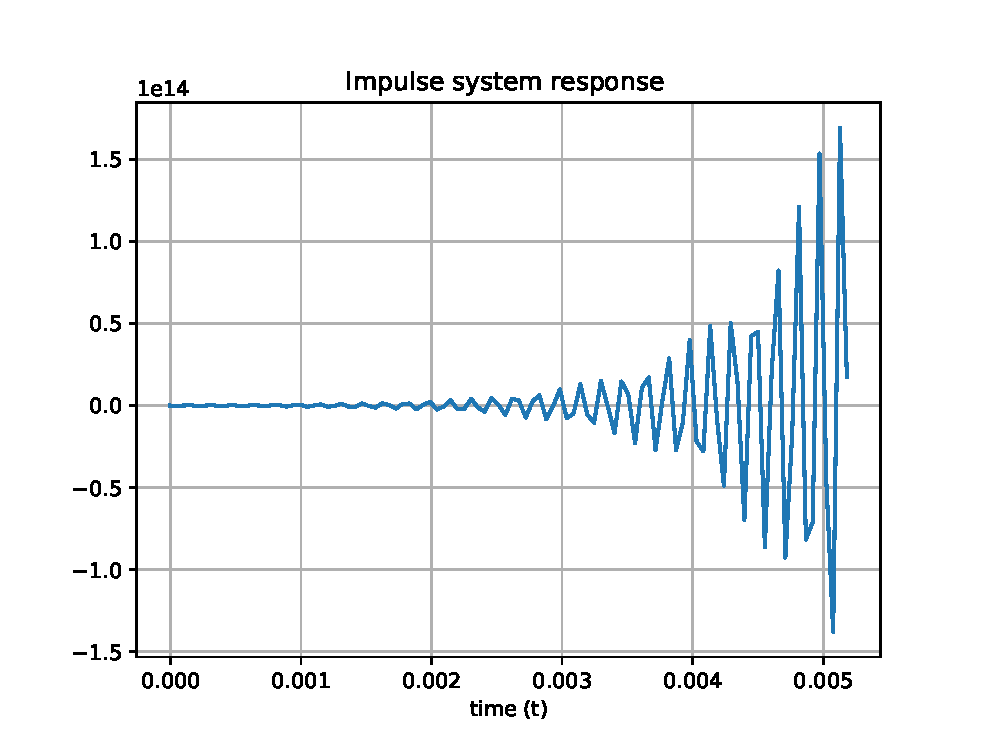
\includegraphics[width=\columnwidth]{./figs/ee18btech11051/ee18btech11051_plot1.eps}
\caption{Impulse Response in python}
\label{fig:ee18btech11051_plot1}
\end{figure}

The circuit simulated in Spice can be found in
\begin{lstlisting}
codes/ee18btech11051/spice/ee18btech11051_spice.asc
\end{lstlisting}
and the python code used for plotting the data is
\begin{lstlisting}
codes/ee18btech11051/ee18btech11051_2.py
\end{lstlisting}

\begin{figure}[!ht]
\centering
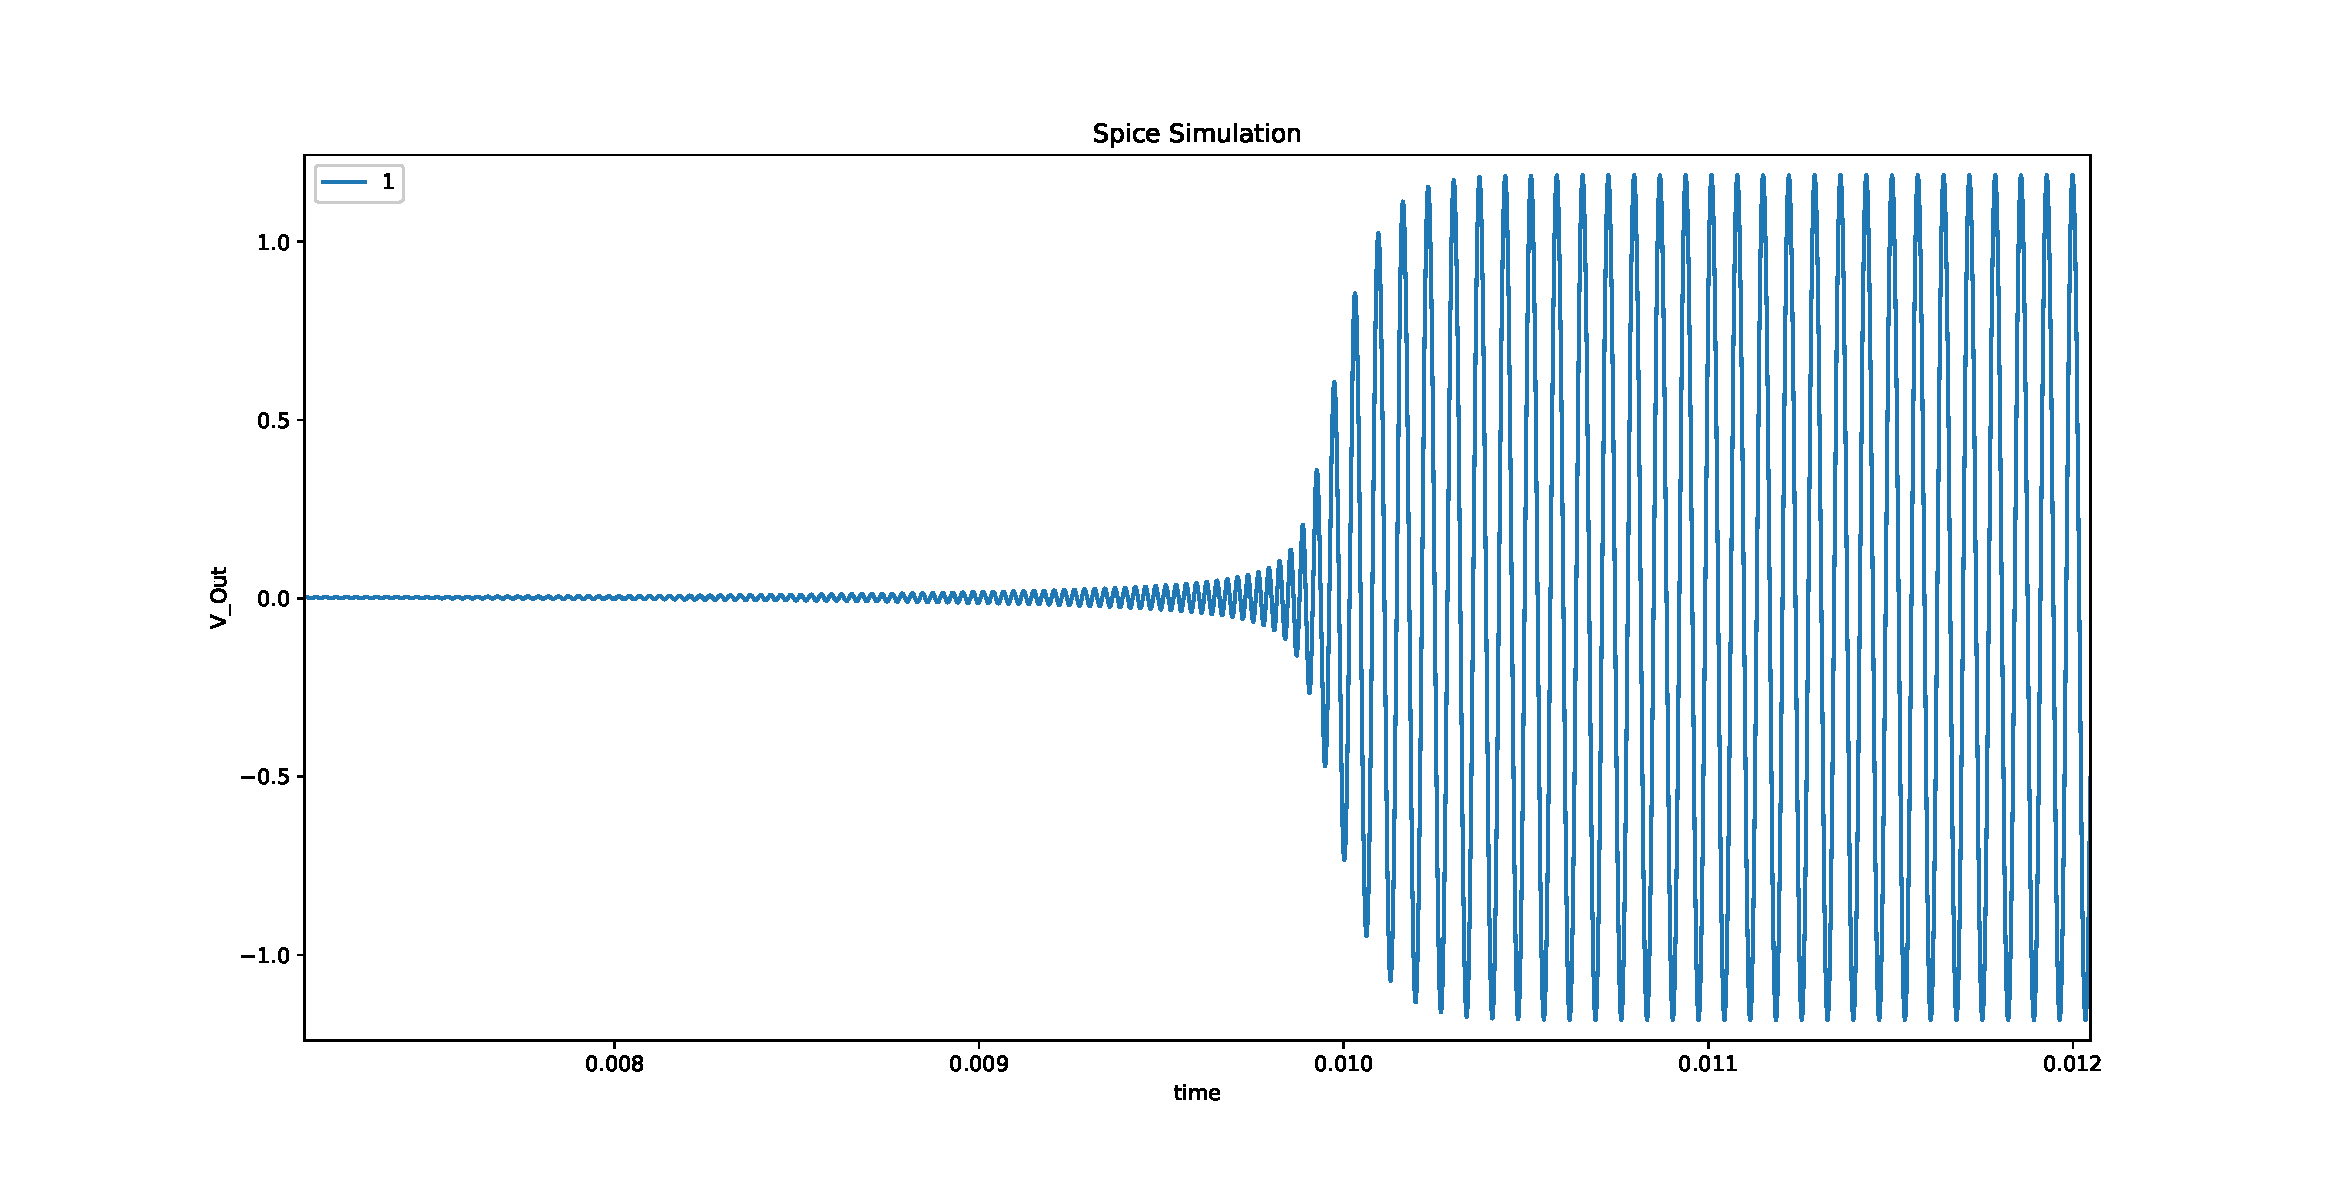
\includegraphics[width=\columnwidth]{./figs/ee18btech11051/ee18btech11051_plot2.eps}
\caption{Spice Simulation}
\label{fig:ee18btech11051_plot2}
\end{figure}
To verify the frequency of the oscillator, we measure the time lapse between two peaks as shown in fig.\ref{fig:ee18btech11051_plot3}
\begin{figure}[!ht]
\centering
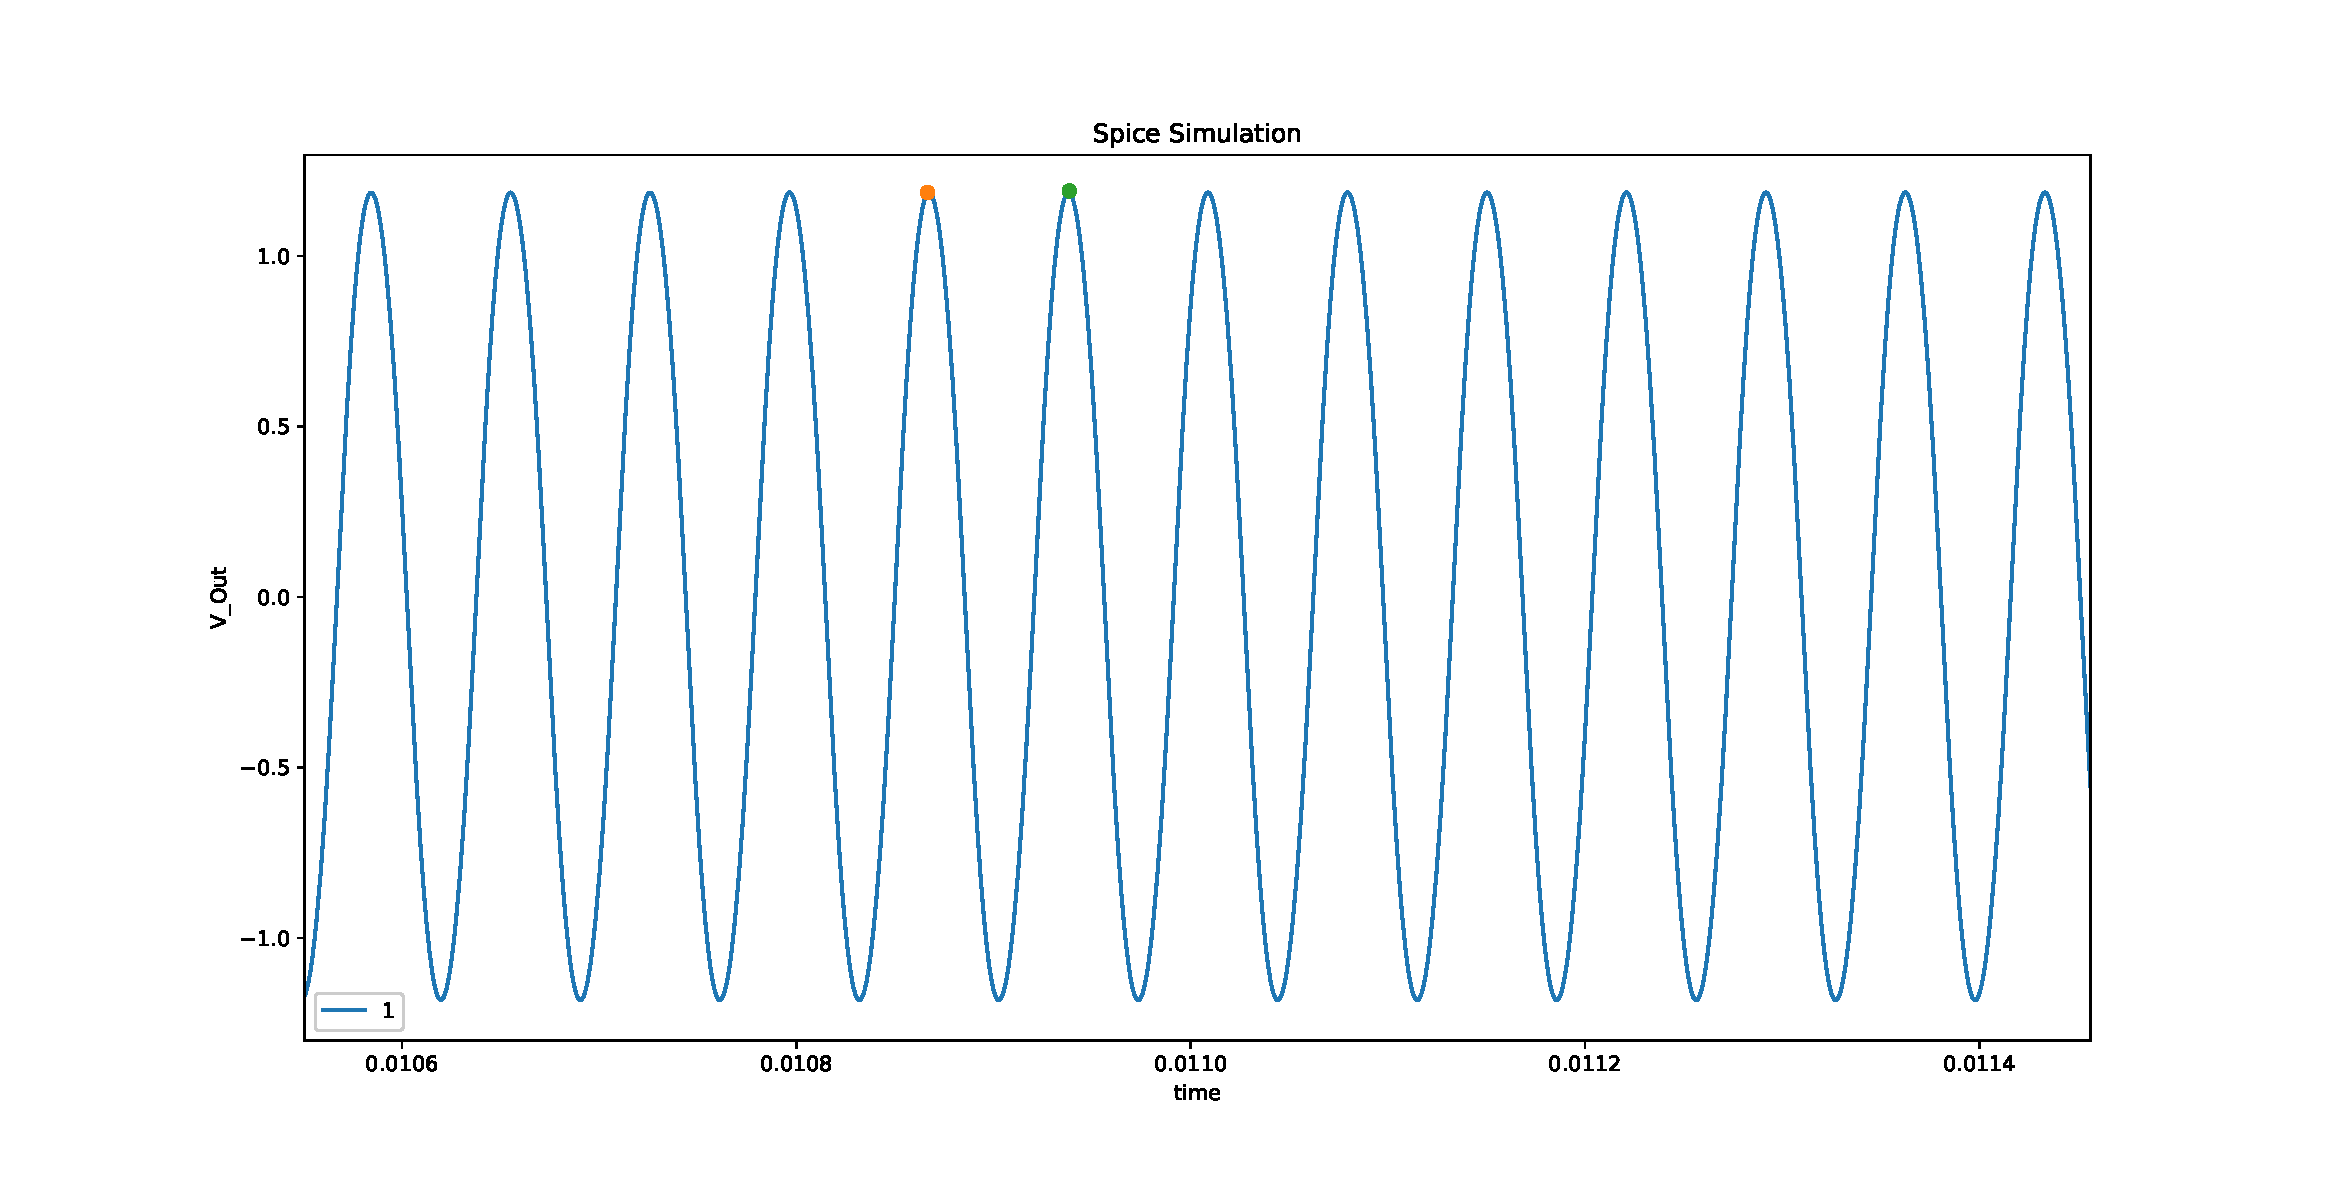
\includegraphics[width=\columnwidth]{./figs/ee18btech11051/ee18btech11051_plot3.eps}
\caption{}
\label{fig:ee18btech11051_plot3}
\end{figure}
The points are (0.0108666, 1.1862) and (0.0109585, 1.1906). So, the time interval between peaks is 0.0109585 - 0.0108666 = 0.0000919.
So, achieved $f_{O} = \frac{1}{0.0000919} = 10.8kHz$.
Hence, the design is achieved.

\end{enumerate}
